\documentclass[tikz]{standalone}
\usepackage{pgfplots}
\pgfplotsset{compat=1.15}
\usepackage{mathrsfs}
\usetikzlibrary{arrows,calc}
\usepackage{tkz-euclide}
\pagestyle{empty}

\definecolor{AngleClr}{rgb}{0,0.39215686274509803,0}
\definecolor{ShapeClr}{rgb}{0.6,0.2,0}
\definecolor{SquareClr}{RGB}{250, 248, 217}

\begin{document}

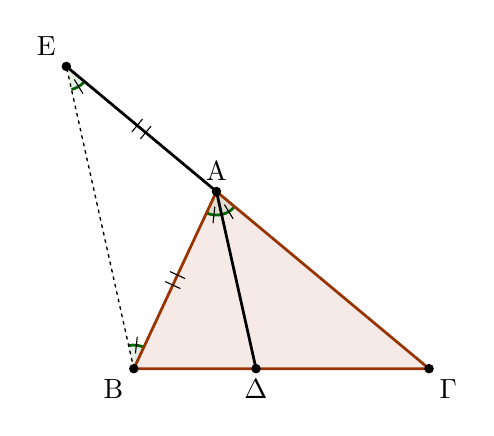
\begin{tikzpicture}[scale=.75]
\tkzSetUpLine[line width=1pt,color=black]
\tkzSetUpPoint[fill=black]

\tkzDefPoints{0/0/B,1.4/3/A,5/0/C}

\tkzDefLine[bisector](B,A,C) \tkzGetPoint{x}
\tkzInterLL(A,x)(B,C) \tkzGetPoint{D}

\tkzDefLine[parallel=through B](A,D) \tkzGetPoint{y}
\tkzInterLL(B,y)(A,C) \tkzGetPoint{E}

\tkzFillPolygon[fill=ShapeClr,fill opacity=0.1](A,B,C)

\tkzFillAngles[fill=AngleClr,size=.4,fill opacity=0.1](B,A,D D,A,C B,E,A A,B,E)
\tkzMarkAngles[line width=1pt,size=.4,color=AngleClr,mark=|,mksize=3](B,A,D D,A,C B,E,A A,B,E)

\tkzDrawSegments[line width=1pt](A,D A,E)
\tkzDrawPolygon[color=ShapeClr](A,B,C)

\tkzDrawPoints[size=3](A,B,C,D,E)

\tkzDrawSegment[line width=0.5pt,color=black,dashed,dash pattern=on 1pt off 1.75pt](B,E)


\tkzLabelPoint[above](A){$\rm A$}
\tkzLabelPoint[below](D){$\rm \Delta$}
\tkzLabelPoint[below left](B){$\rm B$}
\tkzLabelPoint[below right](C){$\rm \Gamma$}
\tkzLabelPoint[above left](E){$\rm E$}

\tkzMarkSegments[mark=||,size=3](A,B A,E)

\end{tikzpicture}

\end{document}
